\chapter{The key exchange problem}
\label{ch:chapter_1}%
This chapter examines solutions to the key-exchange problem. After describing the problem in detail, we present the Diffie-Hellman protocol, alongside its mathematical foundations, being the first effective key-exchange protocol. Then, we explain Shor's algorithm and how it can break the assumptions of DH protocol. Finally, the specific remedy provided by Quantum Key Distribution is introduced.

\section{Before 1976}
The key-exchange problem arises from the need to establish a secure communication channel so that no one but the two endpoints of the channel can obtain a copy of a secret key. That secret key can then be exploited to encrypt the messages exchanged in the communication, making it confidential.

Sharing a secret key is the prerequisite for having confidential communication.

Historically, people had to exchange the key manually to start a secure communication. For example, Julius Caesar had to tell his commanders to shift each letter of a received message to three places to read the original message. He had to communicate this secret in person to remain confidential.

However, nowadays, we want to establish secure communications with entities with which we cannot have a manual exchange. For example, internet communications, which can occur between devices hundreds of kilometers apart, often require to be confidential. How is it possible to agree on a secret key on the internet where anyone can intercept communications?

This problem remained unsolved until 1976, when Diffie and Hellman published their key exchange protocol.

\section{Diffie-Hellman key exchange protocol}
The Diffie-Hellman key exchange protocol \cite{dh76} establishes a shared secret key between two parties. That key can then be exploited to exchange data over a public network (e.g., the internet).

As stated in \cite{hac12}: "Diffie-Hellman key agreement provided the first practical solution to the key distribution problem, allowing two parties, never having met in advance or shared keying material, to establish a shared secret by exchanging messages over an open channel."

\subsection{Protocol description}
Here follows the simplest and original implementation of the protocol, where Alice and Bob are the two entities trying to share a secret key:

\begin{enumerate}
    \item Alice and Bob select and publish a prime number $p$ and an integer number $\alpha$ such that $2 \leq \alpha \leq p-2$;
    \item Alice chooses a secret integer \textit{x}, $1 \leq x \leq p - 2$, computes $\alpha^x\mod{p}$ and sends the result to Bob;
    \item Bob chooses a secret integer \textit{y}, $1 \leq y \leq p - 2$, computes $\alpha^y\mod{p}$ and sends the result to Alice;
    \item Bob receives $\alpha^x$ and computes the shared key as $K = (\alpha^x)^y\mod{p}$;
    \item Alice receives $\alpha^y$ and computes the shared key as $K = (\alpha^y)^x\mod{p}$;
\end{enumerate}

In the end, both Alice and Bob share the very same secret key: $K = \alpha^{xy}\mod{p}$.

\subsection{Protocol security}
Now, we want to discuss the security of the protocol. First of all, let us summarize the public pieces of information that would be available to an attacker, Eve:

\begin{itemize}
    \item The chosen prime number \textit{p};
    \item The chosen integer number $\alpha$;
    \item the message sent to Bob: $\alpha^x\mod{p}$;
    \item the message sent to Alice: $\alpha^y\mod{p}$.
\end{itemize}

In order to break the security of the protocol, Eve should be able to exploit the above public messages to build the secret key. In other words, the attacker should be able to solve the so-called \textit{Diffie-Hellman problem} (DHP), which states that:

\begin{proposition}
Given a prime number \textit{p}, an integer number $2 \leq \alpha \leq p-2$, two integer numbers $1 \leq x, y \leq p -2$ and:
\begin{equation*}
    a = \alpha^x \mod{p}
\end{equation*}
\begin{equation*}
    b = \alpha^y \mod{p}
\end{equation*}
find \textit{c} such that:
\begin{equation*}
    c = \alpha^{xy} \mod{p}
\end{equation*}

\end{proposition}

In cryptography, the DHP is assumed to be computationally hard. Even using the fastest classical computers and the fastest known algorithms, the value of \textit{c} cannot be found with the above publicly-known data.

It can be shown that the DHP is not more complex than the integer factorization problem: given an integer N, which are its prime factors? Indeed, an efficient algorithm able to find the prime factors of N would make it easy to solve the DHP exploiting the Polhig-Hellman algorithm \cite{ph}.

Therefore, solving the integer factorization problem would make the DH algorithm insecure.

An algorithm that can efficiently solve the factorization problem on a classical computer is unknown. However, a quantum algorithm can do it: Shor's algorithm.

\section{Shor's algorithm}
In 1994, Peter Shor proposed the factoring quantum algorithm \cite{shor}, which turns out to simplify the resolution of the integer factorization problem. Indeed, while factorization with classical computers requires a number of steps growing exponentially with the size of the input, the execution of Shor's algorithm is polynomial for the number of digits of the integer to be factored.

According to IBM \cite{ibm}, the longest integer ever factored is 232 digits long, and it required $10^{30}$ operations to be factored. A quantum computer executing Shor's algorithm would factor the same integer with $10^5$ operations.

It is known \cite{shor-order} that the complexity of the factorization problem is equivalent to finding the order of an element. The steps of Shor's algorithm are outlined in the chart below.

\begin{figure}[H]
    \centering
    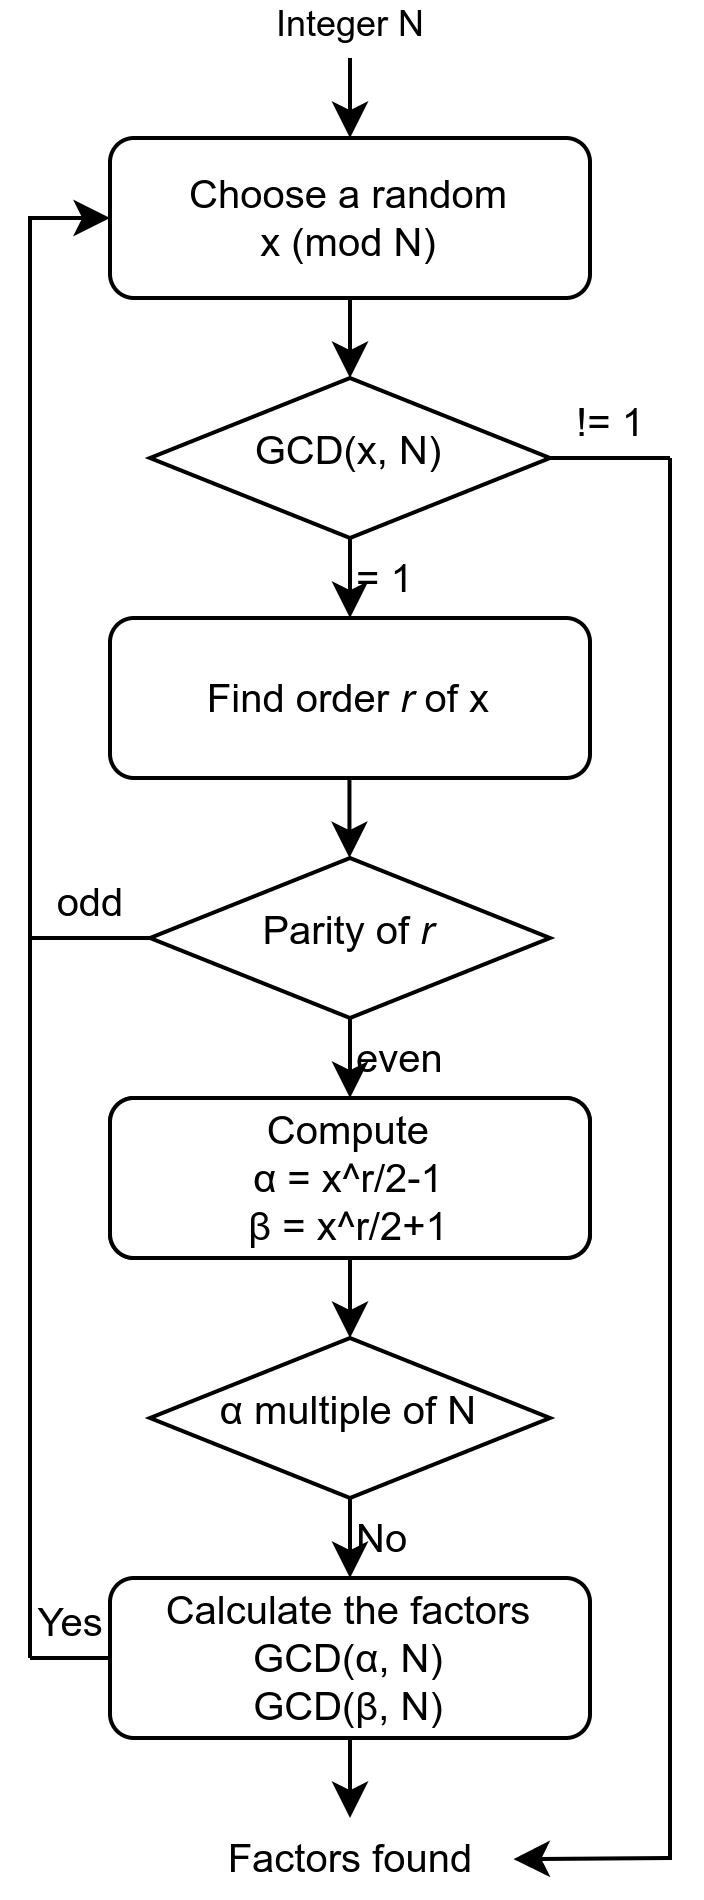
\includegraphics[width=0.4\textwidth]{shor}
    \caption{Shor's algorithm.}
    \label{fig:shor}
\end{figure}

The Greatest Common Divisor (GCD) of two integers is the largest positive integer that divides each integer. Finding GCD is an easy task also for classical computers, exploiting the Euclidean Algorithm \cite{knuth}.

The order \textit{r} is defined as the lowest integer that satisfies $x^r = 1 \pmod N$, and its finding is the bottleneck of classical computers. Shor, instead, showed that the problem could be solved in polynomial time by a quantum computer, drastically reducing the complexity of the overall factorization problem.

When a quantum computer capable of executing Shor's algorithm is available, the security assumptions of the DH algorithm will be compromised. Therefore, cryptographers devised a "quantum-resistant" algorithm for exchanging secret keys: Quantum Key Distribution.

\section{Quantum Key Distribution}
Quantum Key Distribution (QKD) refers to the generation of a secret key between two parties promising information-theoretical security, based on the fundamental laws of quantum mechanics: the algorithm's security does not depend on the computational power of the adversary. Therefore, these protocols can overcome the quantum computation's threat.

An essential and unique feature of QKD is the ability of the two communicating users to detect the presence of any third party aiming at gaining knowledge of the secret key. This capability is a consequence of a fundamental law of quantum mechanics: the process of measuring a quantum system disturbs the system itself. Therefore, a third party that wants to eavesdrop on the secret key must measure it somehow, thus introducing detectable anomalies. In the case of anomaly detection, the two parties abort the key generation process and agree on a new attempt.

The first and most-used QKD protocol is the one proposed by Charles H. Bennett and Gilles Brassard in 1984, known as BB84 \cite{bb84}. Here follows an introduction to the protocol, based on \cite{gagliano}.

\label{ch1:bb84}
In BB84, Alice and Bob are two entities sharing a quantum channel, usually an optical fiber where single-photon signals are transmitted, and an authenticated classical channel. Alice encodes the information on two different polarization bases: diagonal ($D = \{|\nearrow\rangle, |\nwarrow\rangle\}$) or rectilinear ($R = \{|\uparrow\rangle, |\rightarrow\rangle\}$). The protocol follows these steps:

\begin{enumerate}
    \item Alice chooses a random bit string $\beta$ and a random sequence $\pi$ of polarization bases
    \item Alice sends to Bob a train $\phi$ of photons encoded with a polarization state according to this table:
    \begin{table}[H]
    \centering 
        \begin{tabular}{| c | c | c |}
        \hline
        $\beta[i]$ & $\pi[i]$ & $\phi[i]$\\
        \hline \hline
        0 & D & $|\nearrow\rangle$\\\hline
        0 & R & $|\rightarrow\rangle$\\\hline
        1 & D & $|\nwarrow\rangle$\\\hline
        1 & R & $|\uparrow\rangle$\\\hline
        \end{tabular}
    \end{table}
    \item Bob chooses a random sequence $\rho$ of polarization bases
    \item Bob measures the polarization states of $\phi$ according to his choice $\rho$ and interprets the result \textit{r} as shown below:
    \begin{table}[H]
    \centering 
        \begin{tabular}{| c | c | c |}
        \hline
        $\rho[i]$ & $\phi[i]$ & $r[i]$\\
        \hline \hline
        D & $|\nearrow\rangle$ & 0\\\hline
        D & $|\nwarrow\rangle$ & 1\\\hline
        R & $|\rightarrow\rangle$ & 0\\\hline
        R & $|\uparrow\rangle$ & 1\\\hline
        \end{tabular}
    \end{table}
    \item Alice and Bob communicate their respective sequences of polarization bases through the authenticated classical channel.
    \item Both parties retrieve the \textit{sifted key}, discarding from $\beta$ and \textit{r} the bits measured by Bob with incorrect basis. The sifted key is composed only of bits encoded and detected with the same basis. Therefore, the number of correct bits cannot be determined a priori.
    \item Alice and Bob select a random sample of the sifted key to estimate the Quantum Bit Error Rate (QBER), which is the ratio between the number of wrong bits of the sifted key and the length of the sifted key. If the QBER is over an agreed threshold, the sifted key is considered insecure and discarded.
    \item Otherwise, Alice and Bob get the final secret key by applying classical post-processing algorithms to the sifted key, such as information reconciliation (for error correction) and privacy amplification \cite{privacyamp} (for the secretness of the key, guaranteeing that Eve cannot acquire any information about the key). The obtained key is the result of the QKD process.
\end{enumerate}

QKD relies on the fundamental properties of quantum mechanics. In contrast, DH key exchange and other classical protocols are based on the computational complexity of some mathematical problems.

Like all the other key exchange algorithms, QKD is only used to produce a secret key, not transmit any message data. Moreover, it does not offer authentication out of the box: it only focuses on the confidentiality of the secret key.

\label{ch1:length}
The secret key produced by a QKD algorithm is a sequence of bits whose length cannot be established a priori. Indeed, the sifted keys produced by Alice and Bob may differ in some positions due, for instance, to the non-ideality of the experimental realization or dark counts in the single-photon detection. These differences have to be discarded. Moreover, the length of the sifted key may be reduced by the classical post-processing algorithms mentioned above. Therefore, the bits generated by a quantum channel cannot be directly used as a key by encryption algorithms. In the next chapter, we will see how a Key Management Entity faces the problem of creating fixed-length keys exploiting bits produced with QKD.
